%\documentclass[handout]{beamer}
\documentclass{beamer}

\usepackage{bsymb}
\usepackage{b}
\usepackage{xcolor}

% Purpose of modelling?

% difference between axioms and invariants?
% can macine have axioms and vice versa

% why state invariants explicitly
% explain keywords

% ctr := ctr-1  versus  ctr=ctr-1

% explain skip

\mode<presentation>
{
    	%\usetheme{Warsaw}
	\setbeamertemplate{footline}
	{\centerline{\insertframenumber/\inserttotalframenumber}}
} 


\title{More on Event-B: Functions}
\subtitle{Modified and Presented by Andy Edmunds}

\author{\copyright\ Michael Butler}

\institute{ University of Southampton }



\begin{document}



\begin{frame}

\titlepage

\end{frame}














\begin{frame}

\frametitle{Partial Functions}

Special kind of relation:
each domain element has \alert{at most one range element }associated with
it. 

~

To declare $f$ as a partial function:
\[
     \mbox{\fbox{$~f ~\in~ X\pfun Y~$}}
\]

This says that $f$ is a \alert{many-to-one} relation

~

Each domain element is mapped to  \alert{one} range element:
\begin{eqnarray*}
    x~\in~ dom(f) ~
    &~~\implies~~& card(~f[\set{x}]~) ~=~ 1
\end{eqnarray*}

More usually formalised as a \alert{uniqueness} constraint
\begin{eqnarray*}
    x\mapsto y_{1}~\in~ f ~~\land~~ x\mapsto y_{2}~\in~ f
    &~~\implies~~& y_{1} = y_{2}
\end{eqnarray*}

\end{frame}



\begin{frame}


\frametitle{Function Application}

We can use \alert{function application} for partial functions.

~


If $x\in \dom(f)$, then we write ~~~\fbox{$f(x)$}~~~ for the
\alert{unique} range element associated with $x$ in $f$.

~

If $~x\not\in\dom(f)~$, then $f(x)$ is \alert{undefined}.

~

If $~card(~f[\set{x}]~)>1~$, then $f(x)$ is \alert{undefined}.

\end{frame}




\begin{frame}

\frametitle{Examples}

\[
\begin{array}{rcl}
    dir1 & = &
    \set{~  mary \mapsto 398620, \\
&&  ~~jim \mapsto 493028, \\
&&  ~~jane \mapsto 493028 ~}
\end{array}
~~~~~~
\begin{array}{rcl}
    dir2 & = &
    \set{~ mary \mapsto 287573, \\
&&  ~~mary \mapsto 398620, \\
&&  ~~jane \mapsto 493028 ~}
\end{array}
\]

Types of $dir1, dir2$ ? \hspace{0.3cm} $dir1(jim)$ ? \hspace{0.3cm} 
$dir1(sarah)$ ? \hspace{0.3cm} $dir2(mary)$ ? 
~
\pause
~
\vspace{0.5cm}
\begin{description}  \setlength{\itemsep}{4pt}
\centering \item    $dir1 ~\in~ Person \pfun Phone$
\item $dir2 ~\not\in~ Person \pfun Phone$
\pause
 \item $dir1(jim) ~=~ 493028$ 
\item  $dir1(sarah)$ ~is undefined 
\item $dir2(mary)$ is undefined
\end{description}


\end{frame}






\begin{frame}

\frametitle{Well-definedness and application definitions}

\begin{center}
\begin{tabular}{|c|c|}
\hline
Expression & Well-definedness condition \\[2pt] \hline
~&\\
$~~ f(x) ~~$ &  $~~x\in dom(f) ~\land~  f\in X \pfun Y ~~$  \\
~&\\ \hline\end{tabular}
\end{center}

~

The following definition of function application assumes that $f(x)$ is well-defined:

\begin{center}
\begin{tabular}{|c|c|}
\hline
Predicate & Definition \\[2pt] \hline
~&\\
$~~y = f(x) ~~$ &  $~x \mapsto y \in f~$  \\
~&\\ \hline\end{tabular}
\end{center}


\end{frame}





\begin{frame}

\frametitle{Function Operators}

All the \alert{relational operators} can be used on  functions
(restriction, subtraction, image, composition, etc).

~

Be \alert{careful} with some operators!

~

Suppose that $f$ and $g$ are functions.

\begin{itemize}
\item Set Union:~ $f \cup g$ is a  function provided
\[
    x\in \dom(f) ~\land~ x\in \dom(g) ~~~\implies~~~ f(x) = g(x)
\]
Why?


\item Inverse:~ $f^{-1}$ is not always a  function. Why
not?

\item What about $f;g$ ? 
\end{itemize}


\end{frame}




\begin{frame}


\frametitle{Function Overriding}

 \alert{Override} $f$ by $g$ ~~\fbox{~$f\ovl g$~}

~

 $f$ and $g$ must be partial functions of the \alert{same type}

~

Override: \alert{replace}  existing mappings with new ones


%
\begin{eqnarray*}
    dir1 & = &
    \set{~  mary \mapsto 398620, ~  john \mapsto 829483, \\
&& ~~~ jim \mapsto 493028, ~  jane \mapsto 493028 ~}
\end{eqnarray*}
\begin{eqnarray*}
dir1  \ovl   \set{~  mary \mapsto 674321 }  &=& ? \\ &\\
dir1  \ovl   \set{~  mary \mapsto 674321,~  jane \mapsto 829483 }  &=& ? \\\end{eqnarray*}

\end{frame}



\begin{frame}

\frametitle{Function Overriding Definition}

Definition in terms of function \alert{override} and \alert{set union}:

\pause
\begin{eqnarray*}
     f \ovl \set{a \mapsto b} &=&
     (\set{a}\domsub f) \cup \set{a \mapsto b} \\ &\\
     f \ovl g &=&
     (\dom(g)\domsub f) \cup g
\end{eqnarray*}
\end{frame}



\begin{frame}


\frametitle{Birthday Book Example}

Birthday book relates people to their birthday.

~

Each person can have at most one birthday.

~

People can share birthdays.

~

\setsA{
     PERSON ~~~  DATE
}

~

\variablesA{birthday}
%
\invariantA{
        birthday ~\in~ PERSON \pfun DATE   }

~

\initialisationA{
    birthday ~:=~ \set{} }

\end{frame}




\begin{frame}

\frametitle{Adding and checking birthdays}

~

\textit{Add} an entry to the directory: 
\pause
\operA{AddEntry}{
    \anyB{p,d}{p \in Person \\ 
						p\not\in dom(birthday)\\
		d\in Date}{birthday ~\assign~ birthday \cup \set{p\mapsto d}  }
    }

~

\alert{Check} a person's birthday:
\pause
\operA{Check}{
    \anyBs{p,d!}{ p\in dom(birthday) \\ d! = birthday(p)  }
    }


\end{frame}



\begin{frame}

\frametitle{Modifying a birthday}

\alert{Modify} an entry in the directory: 
\pause
\operA{ModifyEntry}{
    \anyB{p,d}{p \in dom(birthday) \\ d\in Date}{birthday ~\assign~ birthday \ovl \set{p\mapsto d}  }
    }

\alert{Syntactic shorthand:} \operA{ModifyEntry}{
    \anyB{p,d}{p \in Person \\ d\in Date}{ \alert{birthday(p) ~\assign~ d}  }
    }


\end{frame}





\begin{frame}


\frametitle{Function inverse}

Check birthdays on a particular date:
\operA{Who}{
    \anyBs{d,ps!}{d \in Date  \\ ps! = birthday^{-1}(d)  }
    }


\begin{itemize}
\item Is this mathematically valid? \pause
\item No:  $ birthday^{-1}$ might not be a function.
\end{itemize}




\end{frame}




\begin{frame}

$ birthday^{-1}$ is a relation:
\[
birthday^{-1} ~~\in~~ Date \rel Person
\]


\frametitle{Function inverse}

Check birthdays on a particular date:
\operA{Who}{
    \anyBs{d,ps!}{d \in Date  \\ ps! = birthday^{-1}[\set{d}]  }
    }


~

Alternative:
\operA{Who}{
    \anyBs{d,ps!}{d \in Date  \\ ps! = dom(birthday\ranres\set{d})  }
    }



\end{frame}





\begin{frame}


\frametitle{Adding the domain as an explicit variable}


~

\variablesA{birthday, person}
%
\invariant{
        birthday ~\in~ PERSON \pfun DATE \\
	person ~\subseteq~ PERSON \\
	person = dom(birthday)  }

~

\initialisationA{
    birthday ~:=~ \set{}~~~~~~~
	person := \set{}   }

\end{frame}





\begin{frame}

\frametitle{Total Functions}

A total function is a special kind of partial function.
 To declare $f$ as a total function:
\[
    \mbox{\fbox{$~f ~\in~ X \tfun Y~$}}
\]

This means that $f$ is well-defined for every element in $X$,
i.e., $f ~\in~ X\tfun Y$  is shorthand for
\[
    f ~\in~ X\pfun Y  ~~\land~~ dom(f) = X
\]


\end{frame}





\begin{frame}


\frametitle{Modelling with Total functions}

We can re-write the invariant for the birthday book to use total
functions:

~

\variablesA{birthday, person}
%
\invariant{
	person ~\subseteq~ PERSON \\
        birthday ~\in~ person \tfun DATE   }

Using the total function arrow means that we don't need to
explicitly specify that $dom(birthday)=person$.

~


We can use $person$ as a guard instead of $dom(birthday)$:

\operA{Check}{
    \anyBs{p,d!}{ p\in person \\ d! = birthday(p)  }
    }


\end{frame}





\begin{frame}

\frametitle{AddEntry needs to be modified}

~

\textit{Add} an entry to the directory: 
\operA{AddEntry}{
    \anyB{p,d}{p \in PERSON \\ 
						p\not\in person\\
		d\in DATE}{birthday ~\assign~ birthday \cup \set{p\mapsto d} \\
						person := person \cup \set{p}  }
    }



\end{frame}





\begin{frame}

\frametitle{Recap}
\begin{itemize}
\item Function is a special case of a relation.
\item Many-to-one: each domain element mapped to a unique range element.
\item Relation operators apply -- with caution!
\item Funtion override.
\item Total functions
\end{itemize}


\end{frame}



\begin{frame}

\frametitle{Secure database example}



We consider a  secure database. Each object in the database has a
 odata component.

~

Each object has a classification between 1 and 10.

~

Users of the system have a clearance level between 1 and 10.

~

Users can only read and write objects whose classification is no
greater than the user's clearance level.

~

What are the \textit{types, variables, events}?





\end{frame}






\begin{frame}
\frametitle{Types and variables}


\setsA{
     OBJECT ~~~    USER
}
%
\variablesA{object,~ user,~  class,~ clear}
%
\pause
\invariant{
    object ~\subseteq~ OBJECT ~\\
    user ~\subseteq~ USER ~\\
        class ~\in~ object \tfun (1..10) ~\\
        clear ~\in~ user \tfun (1..10)
          }

~

\initialisationA{
   object:=\set{}~~~~ user:=\set{}~~~~ class:=\set{}~~~~ clear:=\set{} }

\end{frame}




\begin{frame}
\frametitle{Types and variables}


\setsA{
     OBJECT ~~~  DATA ~~~ USER
}
%
\variablesA{object,~ user,~ odata,~ class,~ clear}
%

\invariant{
    object ~\subseteq~ OBJECT ~\\
    user ~\subseteq~ USER ~\\
       odata ~\in~ object \tfun DATA ~\\
        class ~\in~ object \tfun (1..10) ~\\
        clear ~\in~ user \tfun (1..10)
          }

The \alert{invariant} $odata ~\in~ object \tfun DATA$  means that $odata(o)$ is
well-defined whenever $o\in object$.  ~~ Why is this important?

~

\initialisation{
    object:=\set{}~~~~ user:=\set{}
~~~~odata:=\set{}~~~~ class:=\set{}~~~~ clear:=\set{} }

\end{frame}





\begin{frame}

\frametitle{Adding users}

 \operB{AddUser}{
 \pause
    \anyB{u,c}{
         u ~\in~ USER ~~\\
       u ~\not\in~ user ~~\\
        c ~\in~ 1..10
    }{
        user ~\assign~ user \cup \set{u} \\
        clear(u) ~\assign~ c
    } }

The new user must not already exist.

We need to provide the initial clearance level for the new user.
\end{frame}




\begin{frame}

\frametitle{Adding objects}

\operB{AddObject}{
\pause
    \anyB{o,d,c}{
        o ~\in~ OBJECT  ~~ \\
        o ~\not\in~  object ~~ \\
        d ~\in~ DATA ~\\
		c ~\in~ 1..10
    }{
        object ~\assign~ object \cup \set{o}  \\
        odata(o) ~\assign~ d  \\
        class(o) ~\assign~ c
    } }

The new object must not already exist.

We need to provide the initial classification level and odata value
for the new object.

\end{frame}




\begin{frame}

\frametitle{Reading objects}

 \operB{Read}{
 \pause
    \anyBs{u,o,d!}{ \begin{array}{ll}
        u ~\in~ user ~~  & \mbox{The user must exist} \\
        o~\in~ object ~~ & \mbox{The object must exist}\\
        clear(u) \geq class(o)~~~~  & \mbox{The clearance must be ok} \\
        d! = odata(o)  & \mbox{The odata associated with the object}
           \end{array}
    } }

\end{frame}




\begin{frame}
\frametitle{Writing objects}

 \operB{Write}{
 \pause
    \anyB{u,o,d}{
        u ~\in~ user ~~ \\
        o~\in~ object ~~\\
        clear(u) \geq class(o)
    }{
        odata(o) ~\assign~ d
    } }

    The write operation overwrites the odata value associate with
    the object with a new value.
\end{frame}




\begin{frame}
\frametitle{Changing classification and clearance levels}

\begin{columns}
\begin{column}{2in}
\operB{ChangeClass}{
    \anyB{o,c}{
                o ~\in~ object ~~\\
                c ~\in~ 1..10
    }{
        class(o) ~\assign~ c
    } }
\end{column}
\begin{column}{2in}
 \operB{ChangeClear}{
    \anyB{u,c}{
                u ~\in~ user ~~\\
                c ~\in~ 1..10
    }{
        clear(u) ~\assign~ c
    } }
\end{column}
\end{columns}



\end{frame}




\begin{frame}

\frametitle{Removing users and objects}

\begin{columns}
\begin{column}{2in}
 \operB{RemoveUser}{
 \pause
    \anyB{u}{
        u ~\in~ user
    }{
        user ~\assign~ user \setminus \set{u}  \\
        clear := \set{u} \domsub clear
    } }
\end{column}
\begin{column}{2in}
\pause
 \operB{RemoveObject}{
 \pause
    \anyB{o}{
        o ~\in~ object
    }{
        object ~\assign~ object \setminus \set{o}  \\
        class := \set{o} \domsub class \\
        odata := \set{o} \domsub odata
    } }
\end{column}
\end{columns}


\end{frame}



\begin{frame}
\frametitle{More on Functions}
\begin{center}
\begin{minipage}{0.5\textwidth}
\begin{itemize}
\item $\pinj$ Partial Injection
\item $\tinj$ Total Injection
\item $\psur$ Partial surjection
\item $\tsur$ Total surjection
\item $\tbij$ Bijection
\end{itemize}
\end{minipage}
\end{center}
\end{frame}



\begin{frame}
\frametitle{More on Functions}
\begin{minipage}[t]{0.45\textwidth}
\begin{center}
$\pfun$ Partial function
\begin{figure}
	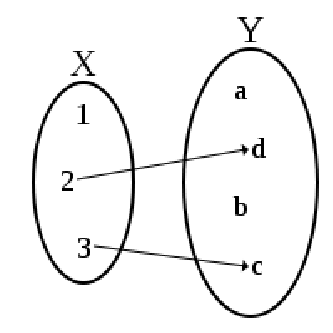
\includegraphics[scale=0.5]{Partial_function}
\end{figure}
Some domain elements not\\
related to range.
\end{center}
\end{minipage}
\begin{minipage}[t]{0.45\textwidth}
\begin{center}
$\tfun$ Total function
\begin{figure}
	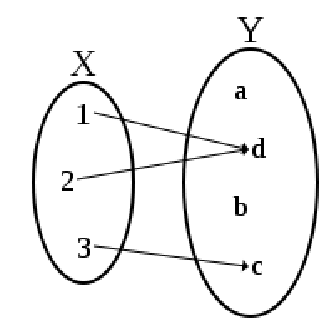
\includegraphics[scale=0.5]{Total_function}
\end{figure}
All domain elements\\
related to range.
\end{center}
\end{minipage}

\end{frame}



\begin{frame}
\frametitle{More on Functions}

\begin{minipage}[t]{0.45\textwidth}
\begin{center}
$\pinj$ Injection
\begin{figure}
	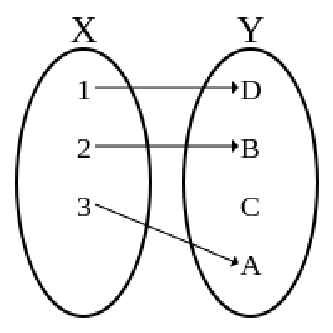
\includegraphics[scale=0.5]{Injection}
\end{figure}
Range elements have a maximum
of one element from the domain.
\end{center}
\end{minipage}
\begin{minipage}[t]{0.5\textwidth}
\begin{center}
$\tinj$ Surjection
\begin{figure}
	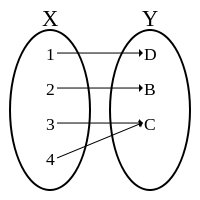
\includegraphics[scale=0.45]{Surjection}
\end{figure}
All range elements are related to the domain by at least one domain element.
\end{center}
\end{minipage}

\end{frame}

\begin{frame}
\frametitle{More on Functions}

\begin{minipage}[t]{\textwidth}
\begin{center}
$\tbij$ (Total) Bijection
\begin{figure}
	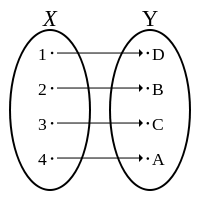
\includegraphics[scale=0.5]{Bijection}
\end{figure}
Every element in the domain is paired in a\\ one-one correspondence with a surjective range.
\end{center}
\end{minipage}
\end{frame}

\begin{frame}
\frametitle{The Lambda Function}
From the Rodin handbook:
\begin{itemize}
\item $(\lambda  p \qdot  P | E )$ is a function that maps an input \emph{p} to a result \emph{E} such that \emph{P} holds.
\item \emph{p} is a pattern of identifiers, parentheses and maplets which follow the following rules:
\begin{itemize}
\item An identfier  \emph{x} is a pattern.
\item An identifier  \emph{x}, followed by an  \emph{oftype} operator is a pattern
\item A pair $a \mapsto b$ is a pattern if \emph{a} and \emph{b} are patterns.
\item  (a) is pattern if a is pattern.
\item In the simplest case, $p$ is just an identifier.
\end{itemize}
\item $(\lambda  p \qdot  P | E ) = \{z\qdot P | p \mapsto E\}$  \\where z is a list of
variables that appear in the pattern p
\end{itemize}

\end{frame}



\begin{frame}
\frametitle{Lambda Examples}
Examples:
\begin{itemize}
\item A function \emph{double} that returns the double value of a natural number:\\
\begin{center}
 $double = (\lambda x \qdot  x \in \nat | 2 * x)$
\end{center}
~

\item The dot product of two 2-dimensional vectors can be defined by:\\
\end{itemize}
\begin{equation}
\begin{split}
dotp = &\\
&(\lambda(a \mapsto b) \mapsto (c \mapsto d) \qdot\\
&\quad a \in \intg \land b \in \intg \land c \in \intg \land d \in \intg | a * c + b * d)
\end{split}
\notag
\end{equation}

\end{frame}



\begin{frame}
\frametitle{Now For Some Practice}

Extend the database specification so that each object has an owner.

~

The clearance associated with that owner must be at least as
high as the classification of the object.  

~

Only the owner of an
object is allowed to delete it.

~

A user's clearance level can only be modified to a new level 
by another user whose clearance level is at least as high as the 
new clearance level.

~

What additional variables are required?

~

What events are affected?
\end{frame}



\end{document}




